\documentclass[a4paper, 11pt, titlepage]{article}
\usepackage{graphicx}
\usepackage{pdfpages}
\usepackage{fancybox}
\usepackage[francais]{babel}
\usepackage[utf8]{inputenc}
% \usepackage[T1]{fontenc}
\usepackage{amsmath,amsfonts,amssymb}
\usepackage{fancyhdr}
\usepackage{stackrel}
\usepackage{babel,indentfirst}
\usepackage{xspace}
\usepackage{url}
\usepackage{titling}
\usepackage{listings}
\usepackage{color}
\usepackage{array}
\usepackage{hyperref}
\usepackage{makecell}
\usepackage{tikz}
\usepackage{float}
\usepackage{wrapfig}

%\setlength{\parindent}{0pt}
\setlength{\parskip}{1ex}
\setlength{\textwidth}{17cm}
\setlength{\textheight}{24cm}
\setlength{\oddsidemargin}{-.7cm}
\setlength{\evensidemargin}{-.7cm}
\setlength{\topmargin}{-.5in}


\lstset{
  sensitive=f,
  morestring=[d]",
  showstringspaces=false,
  basicstyle=\small\ttfamily,
  keywordstyle=\bf\small,
  commentstyle=\itshape,
  stringstyle=\sf,
  extendedchars=true,
  columns=[c]fixed
}



\predate{
\begin{center}
}
\postdate{
\\
\vspace{1.5cm}

\includegraphics[scale=0.7]{imag.png}
\end{center}}


\title {{ {\huge Compte rendu du projet make }} }

\author{\Large Equipe 10 \\
\\
    {\sc Boudouin}~Philippe\\
    {\sc Danet}~Nicolas\\
    {\sc Ferrand}~Pierre\\
    {\sc Gouttefarde}~Léo
}

\date{Vendredi 25 Novembre 2016}

\lhead{Projet Make}
\rhead{Compte rendu}

\begin{document}
\pagestyle{fancy}
\maketitle

\setcounter{tocdepth}{2}

\tableofcontents
\newpage

\section {Présentation du projet}

\subsection {Langage / Framework}

Le projet a été réalisé à l'aide du framework Charm\texttt{++}, qui s'utilise en C\texttt{++}.
Il s'agit d'un framework très complet du même type que Qt mais pour permettre de créer des applications distribuées et multi-coeurs.

Pour cela le framework est basé sur une gestion de l'application par objets distribués et méthodes d'objet distantes, dont la spécification doit être faite dans un format de fichier d'interface dédié (fichiers .ci).
Le framework utilise ainsi un compilateur spécifique.


\subsection {Architecture}

Le projet s'organise autour de différentes classes :

\begin{itemize}

\item[$-$]
\lstinline!Parser! :
Effectue le parsing du Makefile

\item[$-$]
\lstinline!Master! :
Classe de l'objet distribué principal, le maître

Il gère des esclaves, leur transmet des tâches,
et récupère les résultats

\item[$-$]
\lstinline!Slave! :
Classe des objets distribués d'esclaves

Les esclaves reçoivent des tâches du maître qu'ils doivent exécuter,
puis en revoyer le résultat

\item[$-$]
\lstinline!Node! :
Classe des noeuds du graphe de dépendances tiré d'un Makefile

Cette classe permet de gérer les différentes opérations faites sur les noeuds, elle permet aussi de créer le graphe des dépendances à partir des éléments parsés


\item[$-$]
\lstinline!Job! :
Cette classe décrit les tâches envoyées à distance aux esclaves


\item[$-$]
\lstinline!File! :
Cette classe décrit les fichier à envoyer entre objets distribués,
elle définit leur lecture / écriture / transmission

\end{itemize}


\subsection {Algorithme principal}

Le maître envoie des tâches aux esclaves, les esclaves une fois terminé renvoient leur résultat au maître qui regarde alors si une nouvelle tâche à exécuter est disponibles (donc dont toutes les dépendances sont créées).



\subsection {Extensions}

En plus des fonctionnalités de base, notre programme de make permet d'utiliser plusieurs CPUs par machine et minimise les envois de dépendances aux esclaves (on ne renvoie jamais une dépendance précédemment envoyée).

De plus la dernière tâche est effectuée sur le maître pour en accélérer l'exécution (plus besoin de distribuer de tâches à ce moment là).


\subsection {Installation}

\noindent Pour installer Charm\texttt{++}, il faut en récupérer l'archive, la décompresser puis compiler :

\begin{verbatim}
cd ~
wget http://charm.cs.illinois.edu/distrib/charm-6.7.1.tar.gz
tar -xvzf charm-6.7.1.tar.gz
cd ~/charm-6.7.1
./build charm++ netlrts-linux-x86_64 --with-production -j8
\end{verbatim}

Sur Grid'5000, nous stockons ce dossier dans répertoire home et spécifions ce répertoire d'installation dans le Makefile.


\subsection {Déploiement sur Grid'5000}

Le code de déploiement est écrit en bash avec les différentes étapes décrites dans le fichier \texttt{scripts/deploy.sh}.

Pour l'exécution distribuée, Charm\texttt{++} comporte un équivalent à mpiexec : charmrun.


\subsubsection {Etape 1}

Connexion, réservation et installation de 10 noeuds pour 1h par exemple (on installe notamment blender et ffmpeg) :

\begin{verbatim}
ssh <login>@access.grid5000.fr
ssh <site>

oarsub -I -l nodes=10,walltime=1 -t deploy
kadeploy3 -f $OAR_NODE_FILE -e jessie-x64-std -k
\end{verbatim}

\subsubsection {Etape 2}

Préparation des noeuds et installation de Charm\texttt{++} :

\begin{verbatim}
# runs a script remotely
remote_run()
{
  if [[ $# -ge 2 && -f "$2" ]]; then
    ssh -oStrictHostKeyChecking=no root@$1 'bash -s' < "$2"
  fi
}

# Charm++ nodelist file (regenerate it after each oarsub node allocation)
NODELIST=~/nodelist

sort -u $OAR_NODEFILE > nodes

# Generates Charm++ nodelist file
# each line from $OAR_NODEFILE = 1 cpu entry, usually 8 / node
awk '$0="\thost "$0" ++cpus 8"' nodes > tmp
echo "group main" > $NODELIST
cat tmp >> $NODELIST
rm tmp

echo -e "apt-get update\napt-get -y install blender ffmpeg ImageMagick ncftp" > task.sh
echo -e "nohup sh ~/task.sh &> out.txt &" > runTask.sh

SERVS=$(cat nodes)
SSH=$(tail -n 1 nodes)

# for each node
for SERV in $SERVS; do

  scp ~/.ssh/id_rsa root@$SERV:~/.ssh/id_rsa
  scp ~/.ssh/id_rsa.pub root@$SERV:~/.ssh/id_rsa.pub

  scp $NODELIST root@$SERV:~
  scp nodes root@$SERV:~
  scp task.sh root@$SERV:~

  remote_run $SERV runTask.sh

done

ssh root@$SSH

cd ~
wget http://charm.cs.illinois.edu/distrib/charm-6.7.1.tar.gz
tar -xvzf charm-6.7.1.tar.gz
cd ~/charm-6.7.1
./build charm++ netlrts-linux-x86_64 --with-production -j8
\end{verbatim}



\subsubsection {Etape 3}

Içi il faut télécharger l'archive de notre application dans un dossier et la décompresser dans le dossier home, puis changer les identifiants FTP à la fin du fichier test/bench.sh si l'on souhaite que les résultats soient zippés sur un FTP à la fin.


\subsubsection {Etape 4}

Il s'agit maintenant de compiler et de finaliser les noeuds avec les instructions suivantes :

\begin{verbatim}
cd ~/make/src

# Fix Charm++ path
tail -n +4 Makefile >> Makefile_
echo "CPATH=~/charm-6.7.1" > Makefile
cat Makefile_ >> Makefile

make -j8


cd ~/make/sujet/makefiles/premier
gcc premier.c -lm -o premier
cd ~

# for each node
for SERV in $(cat ~/nodes); do
  scp -o StrictHostKeyChecking=no -rp ~/make root@$SERV:~
done
\end{verbatim}


\subsubsection {Etape 5}

Finalement pour lancer le benchmark de test il suffit d'utiliser l'instruction suivante :

\begin{verbatim}
cd ~/make
nohup ./test/bench.sh &> bench.log &
\end{verbatim}


\subsubsection {Etape 5 (mode manuel)}

Pour exécuter le programme sans le script de benchmarking, il faut se mettre dans le dossier du Makefile à tester puis appeler le programme comme ceci :

\begin{verbatim}
~/make/charmrun ++nodelist ~/nodelist ++ppn <Nombre de processus par noeud> \
++p <Nombre de processus total> ~/make/src/Make <FichierMakefile>
\end{verbatim}

Le fichier \lstinline!~/nodelist! contient la liste des noeuds disponibles selon la syntaxe Charm\texttt{++} (créé en étape 2).


\newpage

\section {Tests de performance}

Les tests suivants ont été effectués sur les machines du cluster Edel de Grenoble, avec un maximum de 42 machines.
Les caractéristiques de ces machines sont les suivantes :

\begin{itemize}

\item
2 CPUs Intel Xeon E5520

\item
4 coeurs par CPU

\item
24 GB de RAM

\item
119 GB d'espace disque SSD

\end{itemize}


\subsection {Tests mono-coeurs}




\subsubsection {Blender 2.49}
\subsubsection* {Makefile}

\begin{center}
% \begin{figure}[ht!]
    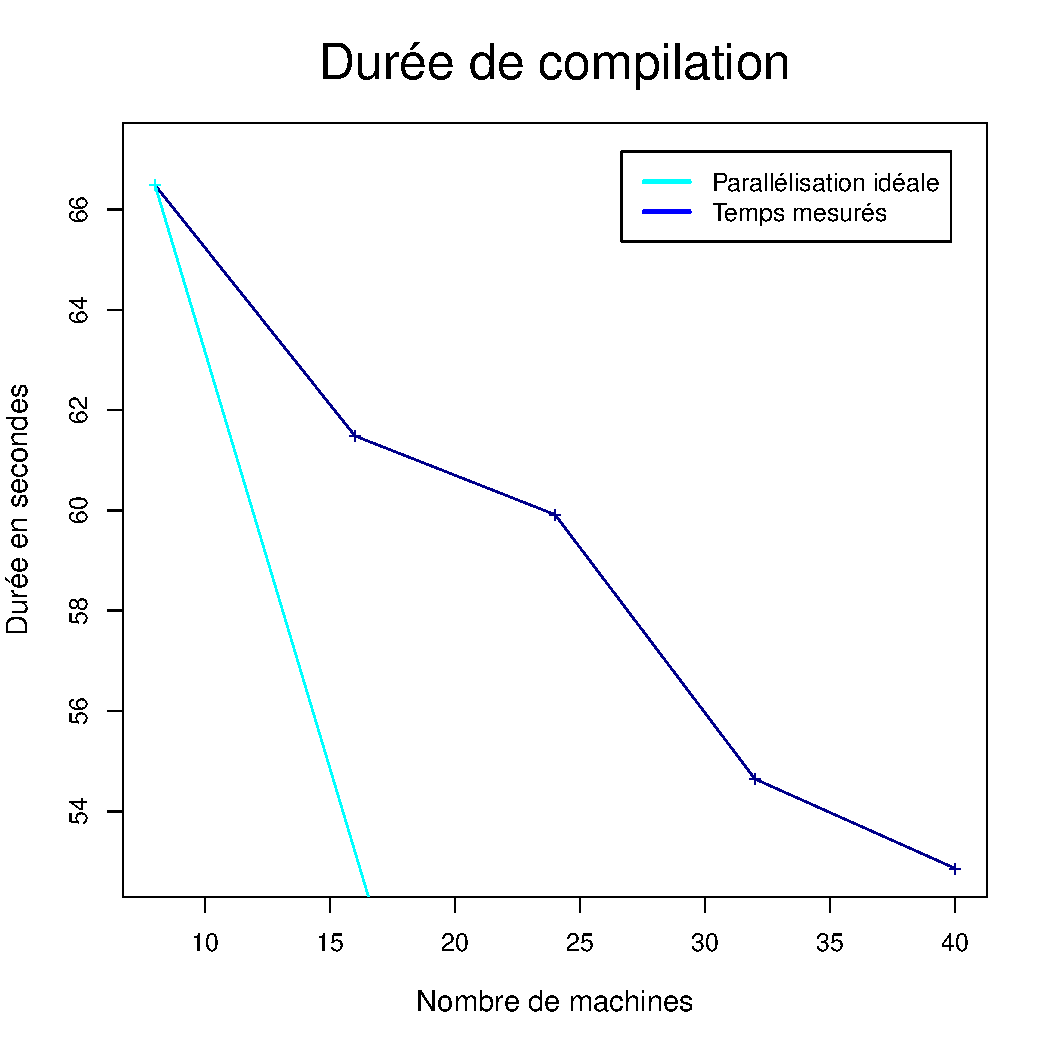
\includegraphics[scale=0.45]{res/sujet_makefiles_blender_249_Makefile_nth1.pdf}
% \caption{Diagramme des cas d'utilisation}
% \end{figure}
\end{center}


\subsubsection* {Makefile-recurse}

\begin{center}
% \begin{figure}[ht!]
    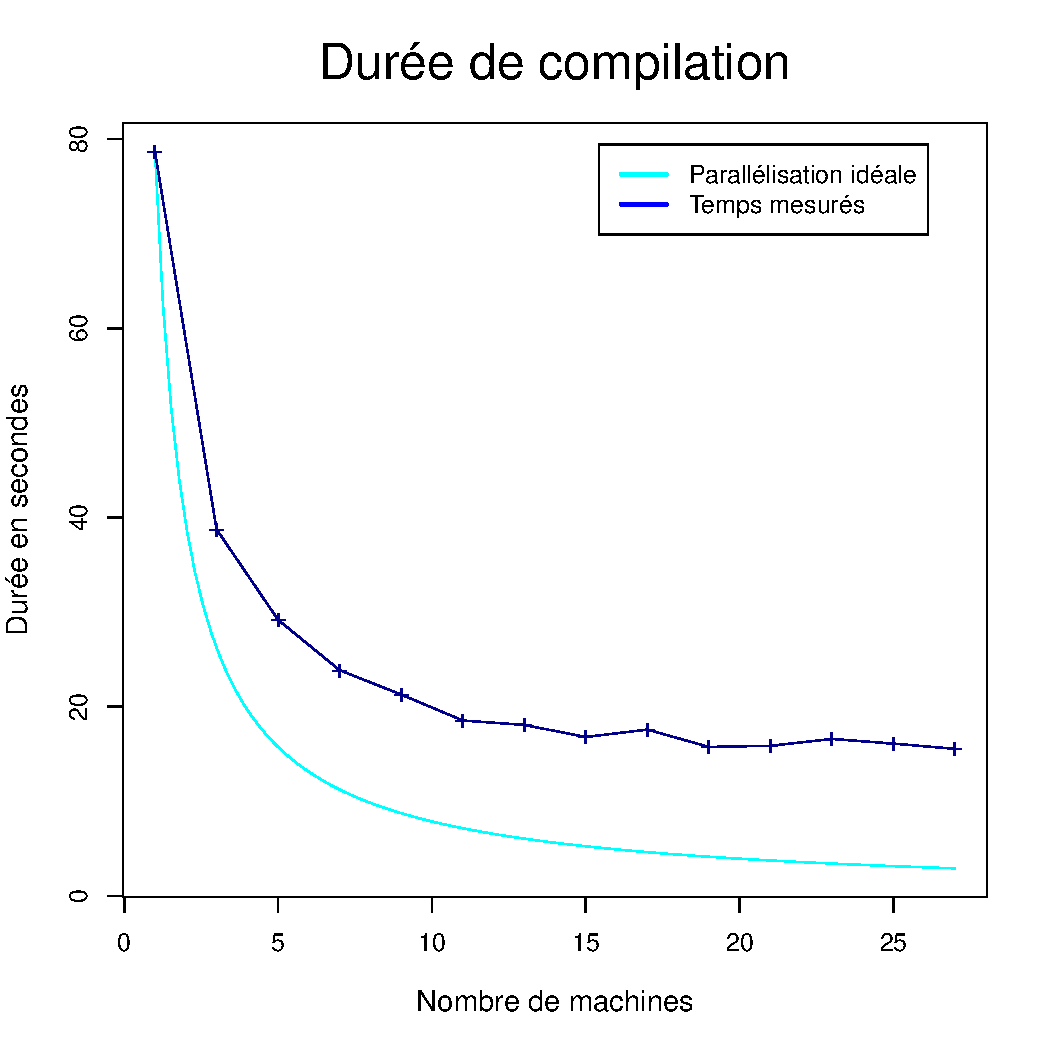
\includegraphics[scale=0.45]{res/sujet_makefiles_blender_249_Makefile-recurse_nth1.pdf}
% \caption{Diagramme des cas d'utilisation}
% \end{figure}
\end{center}


\subsubsection {Blender 2.59}


\begin{center}
% \begin{figure}[ht!]
    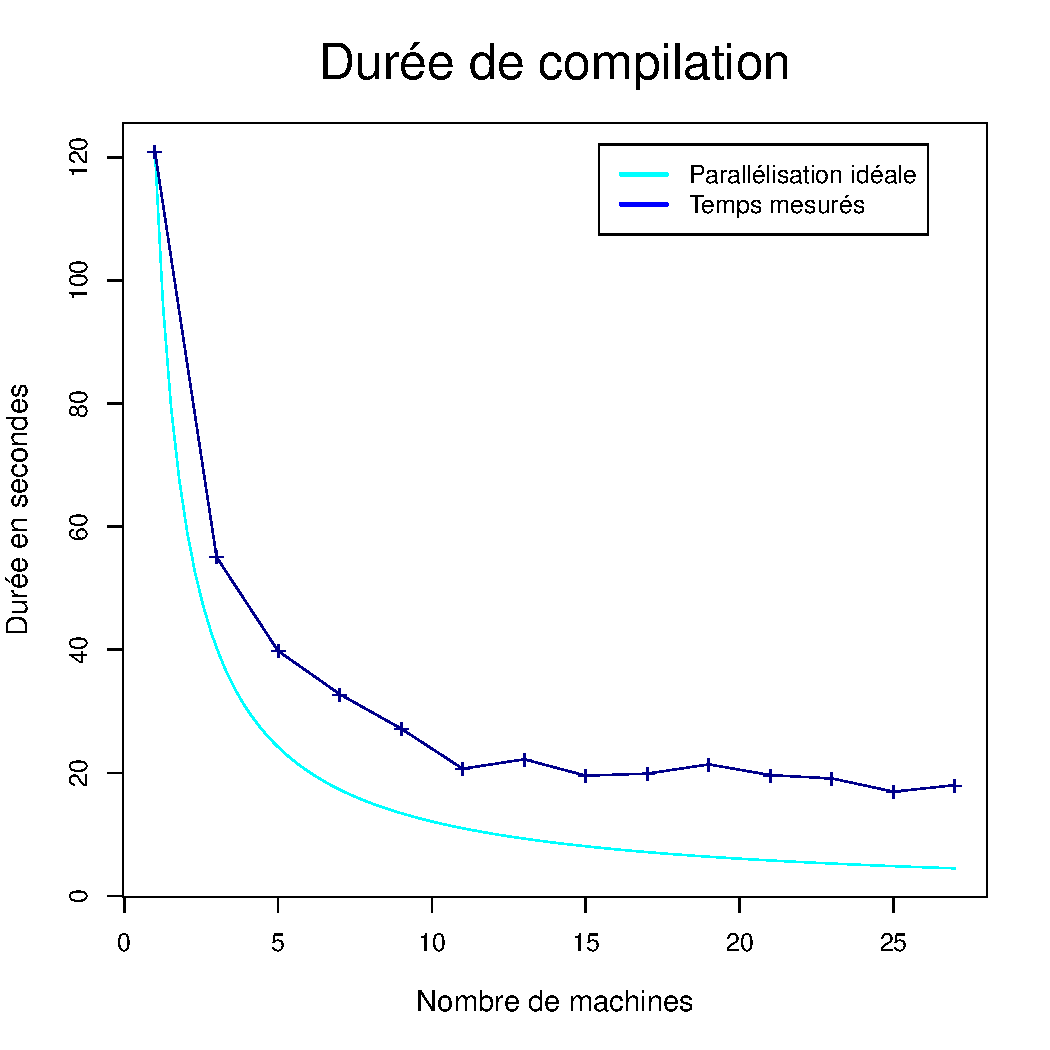
\includegraphics[scale=0.45]{res/sujet_makefiles_blender_259_Makefile_nth1.pdf}
% \caption{Diagramme des cas d'utilisation}
% \end{figure}
\end{center}



\subsubsection {Matrix}

\begin{center}
% \begin{figure}[ht!]
    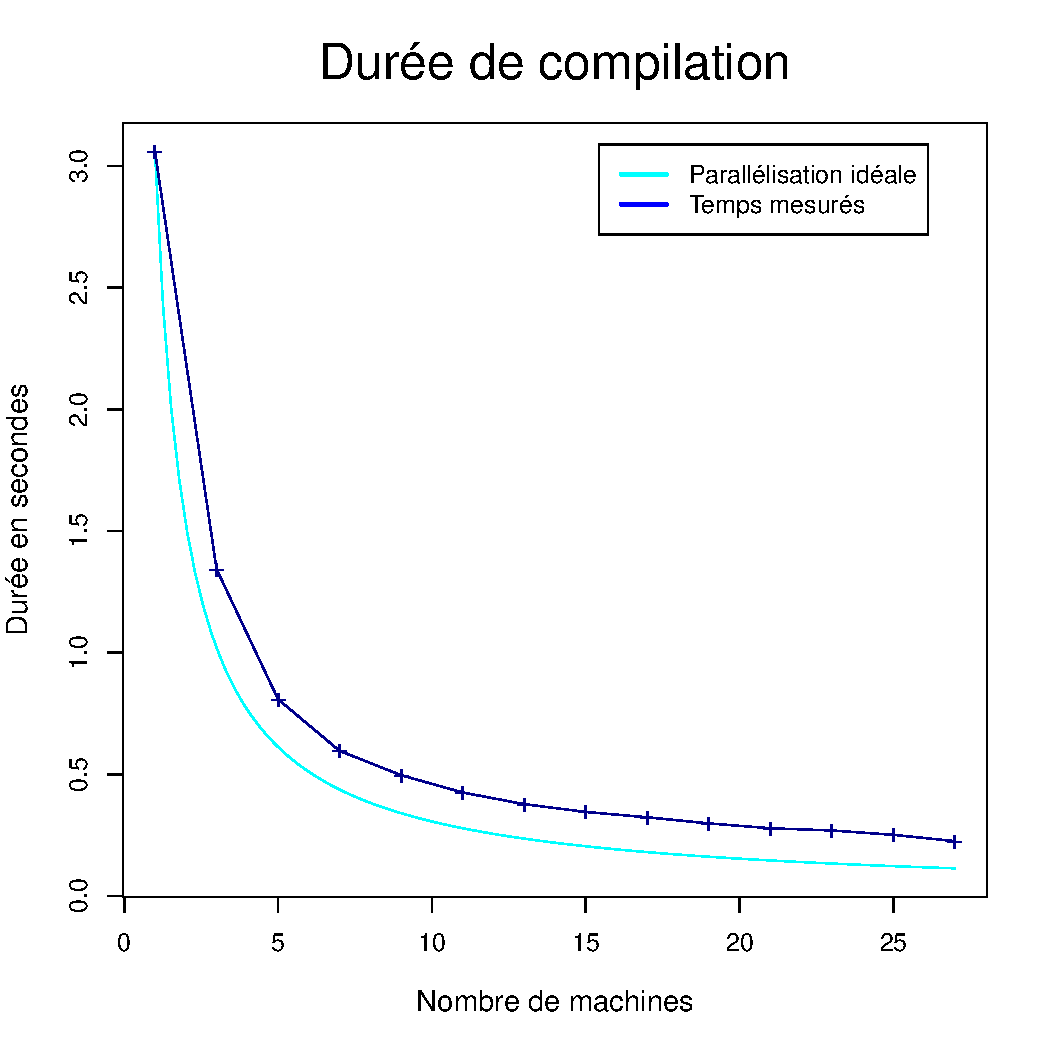
\includegraphics[scale=0.45]{res/sujet_makefiles_matrix_Makefile_nth1.pdf}
% \caption{Diagramme des cas d'utilisation}
% \end{figure}
\end{center}


\subsubsection {Premier}

\subsubsection* {Makefile}

\begin{center}
% \begin{figure}[ht!]
    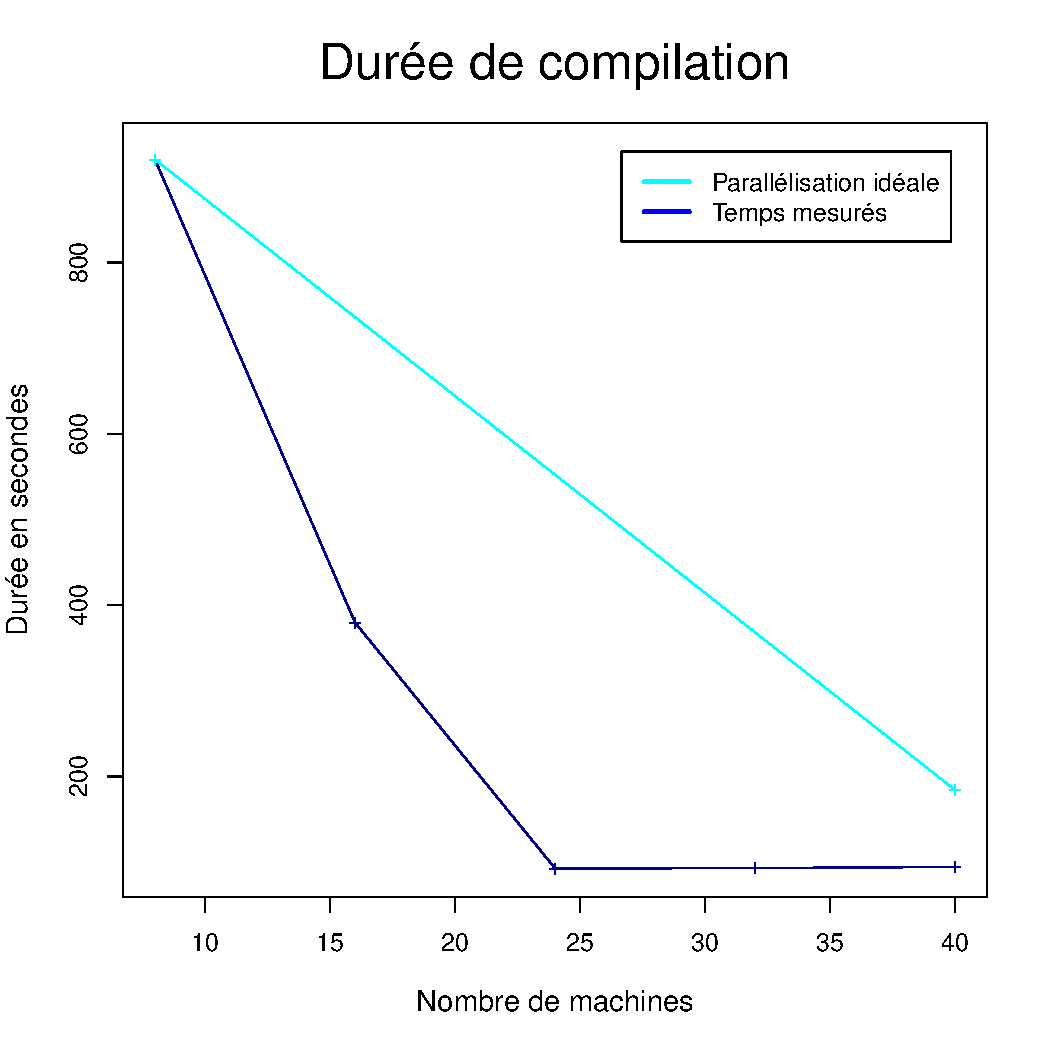
\includegraphics[scale=0.45]{res/sujet_makefiles_premier_Makefile_nth1.pdf}
% \caption{Diagramme des cas d'utilisation}
% \end{figure}
\end{center}


\subsubsection* {Makefile-small}

\begin{center}
% \begin{figure}[ht!]
    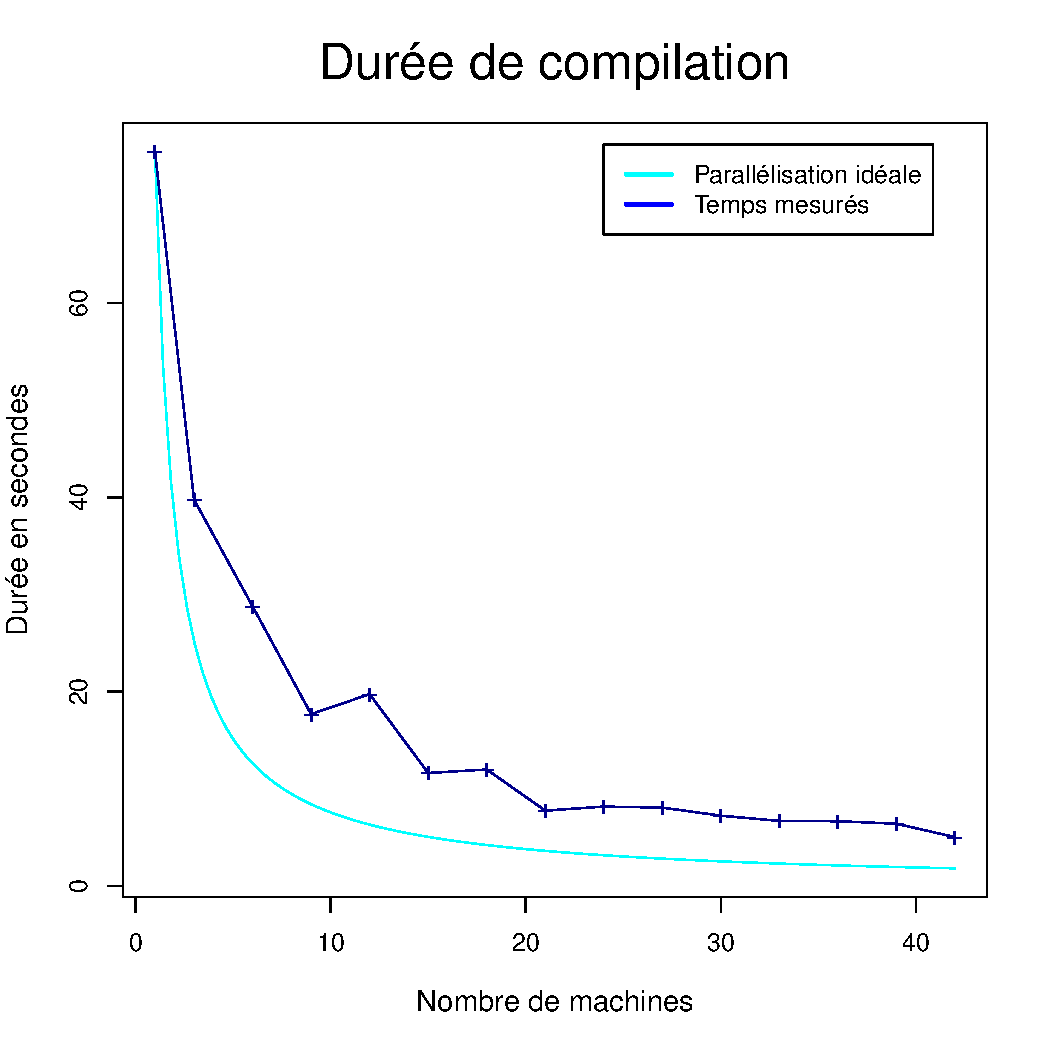
\includegraphics[scale=0.45]{res/sujet_makefiles_premier_Makefile-small_nth1.pdf}
% \caption{Diagramme des cas d'utilisation}
% \end{figure}
\end{center}




\newpage

\subsection {Tests multi-coeurs}

Voici quelques exemples des performances bien meilleures obtenues en exploitant chacun des 8 coeurs (2 x 4 coeurs) disponibles par machine. Nous avons aussi rajouté les courbes d'efficacité et d'accélération pour ces deux exemples.

\subsubsection {Blender 2.49 : Makefile}

\begin{center}
% \begin{figure}[ht!]
    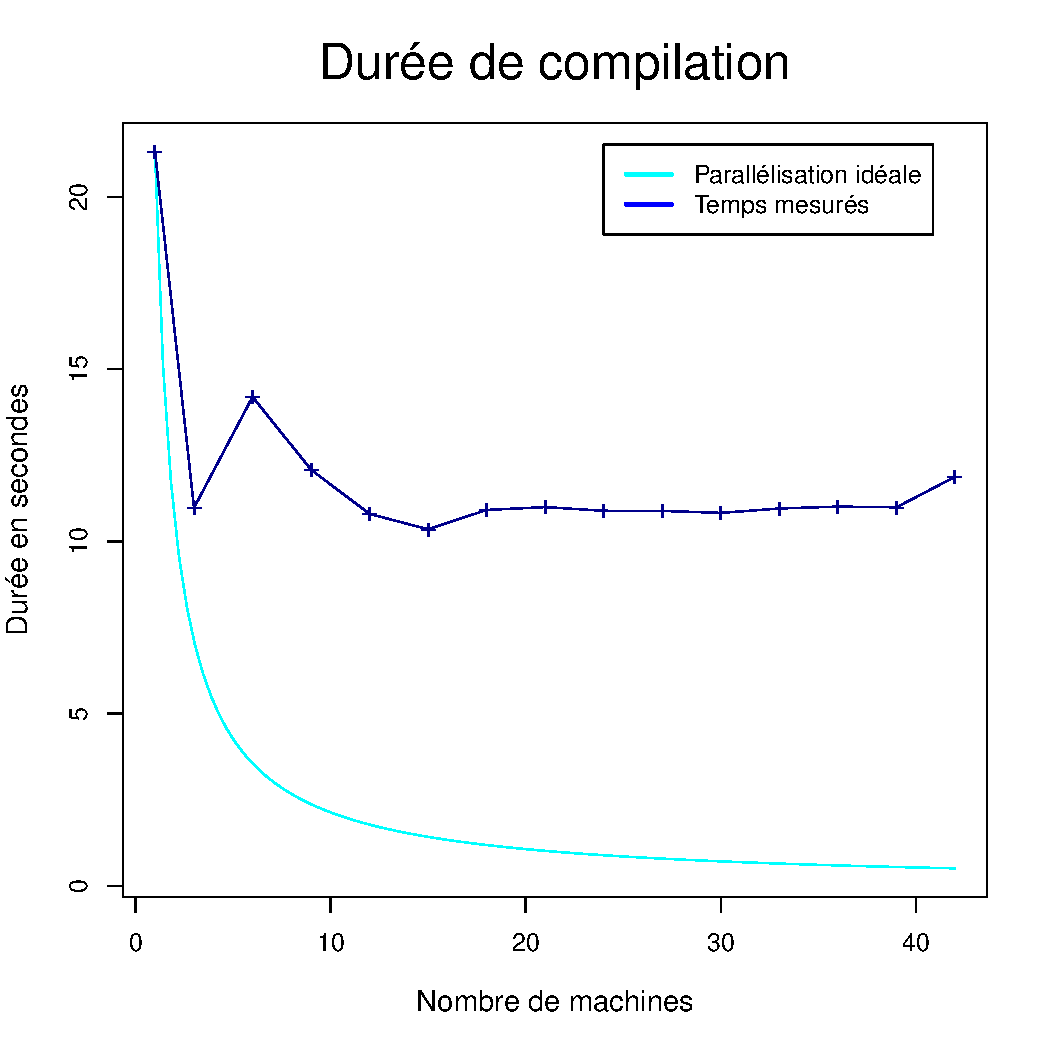
\includegraphics[scale=0.45]{res/sujet_makefiles_blender_249_Makefile_nth8.pdf}
    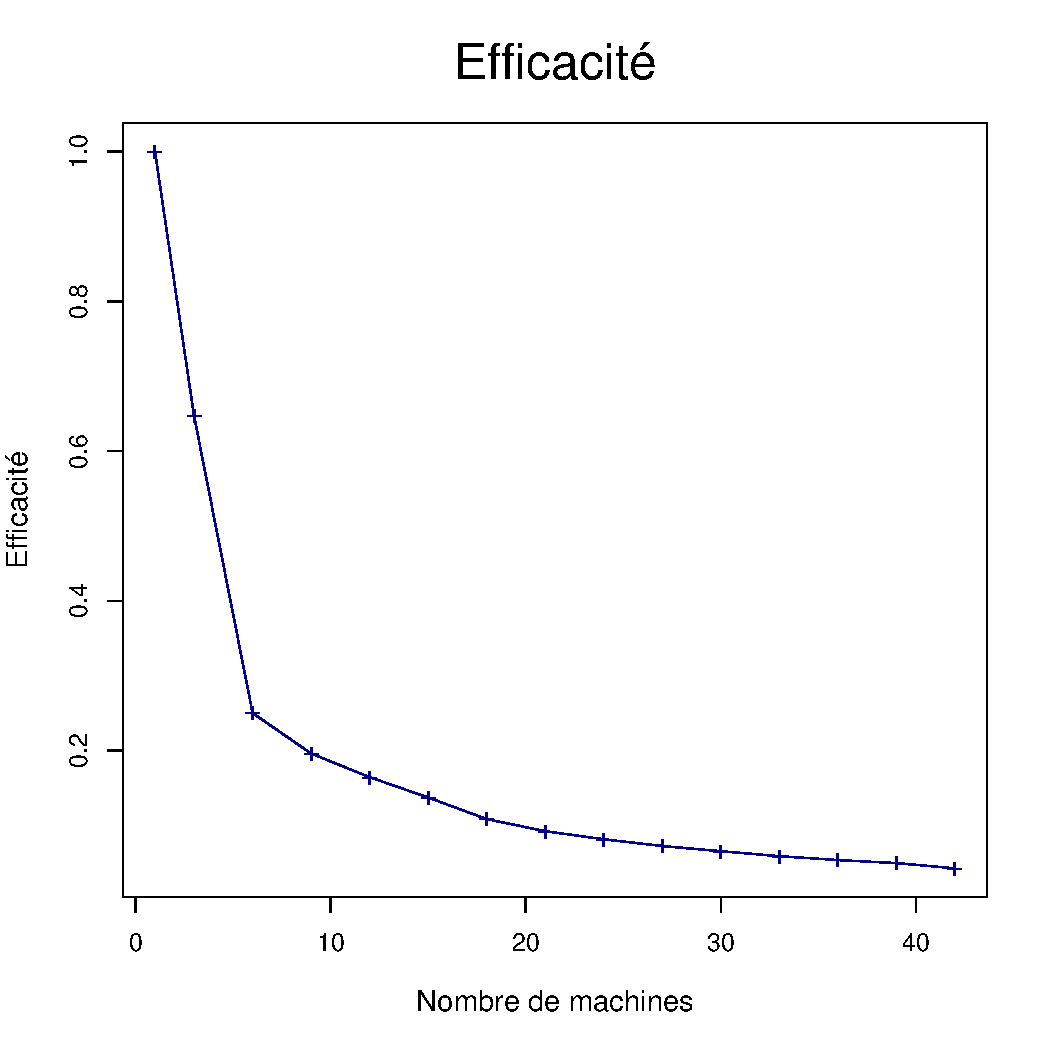
\includegraphics[scale=0.45]{res/sujet_makefiles_blender_249_Makefile_nth8_eff.pdf}
    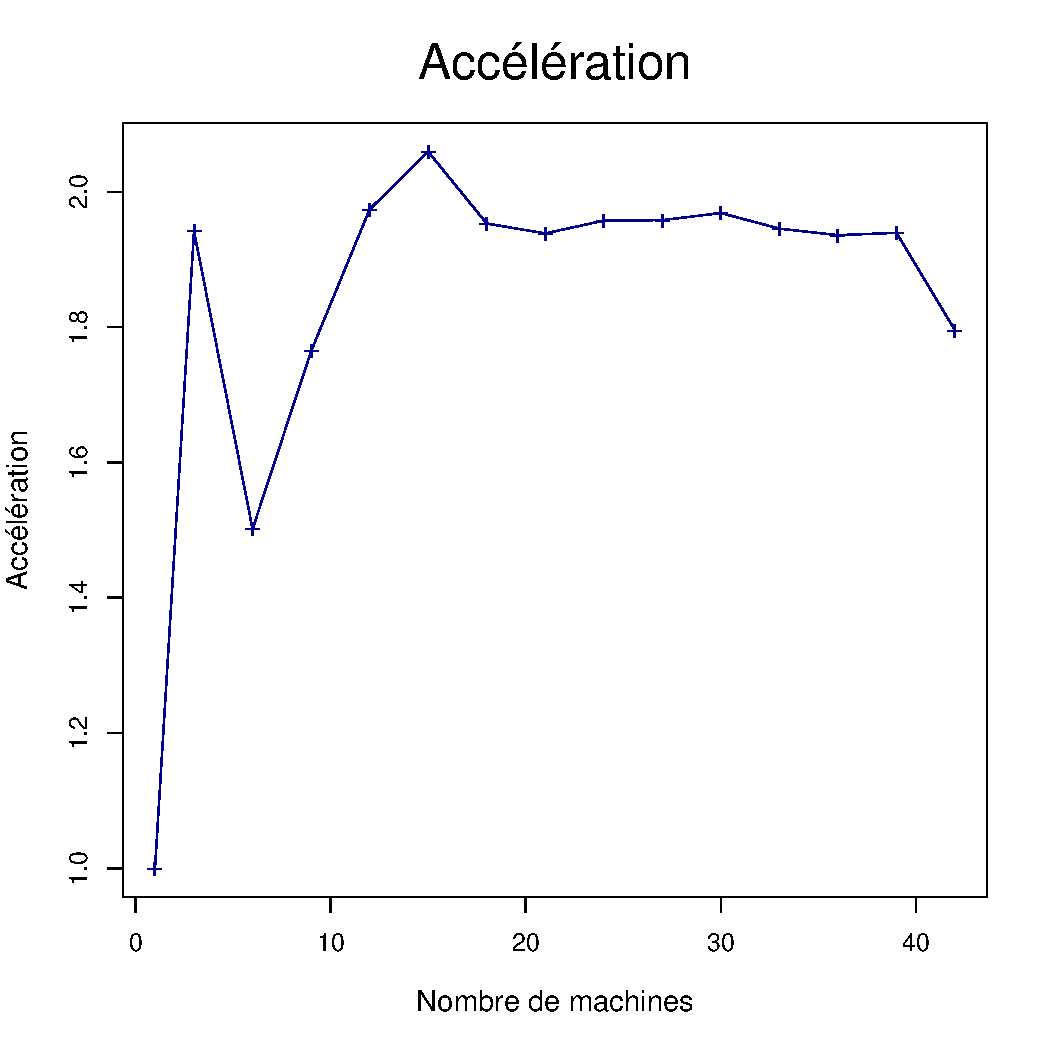
\includegraphics[scale=0.45]{res/sujet_makefiles_blender_249_Makefile_nth8_acc.pdf}
% \caption{Diagramme des cas d'utilisation}
% \end{figure}
\end{center}



\subsubsection {Premier : Makefile}

\begin{center}
% \begin{figure}[ht!]
    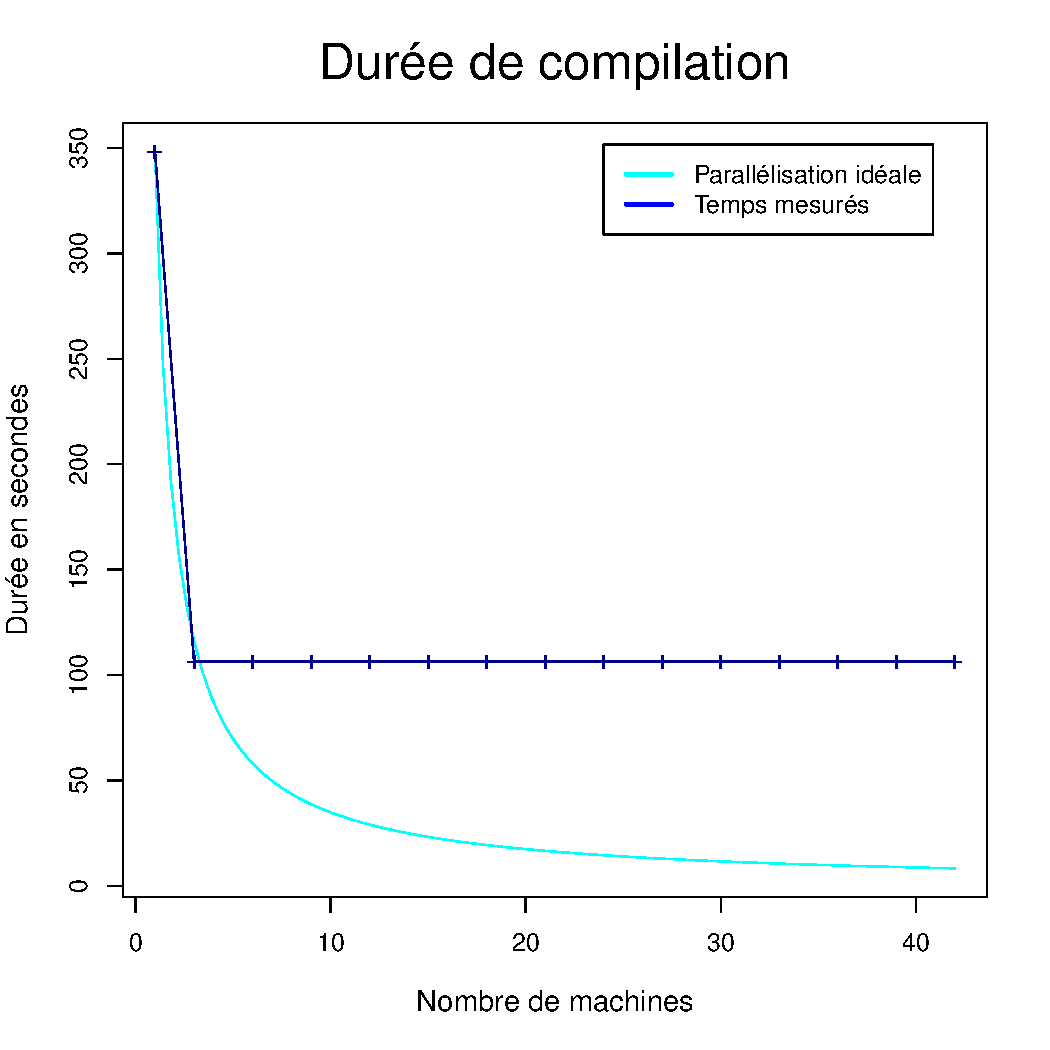
\includegraphics[scale=0.45]{res/sujet_makefiles_premier_Makefile_nth8.pdf}
    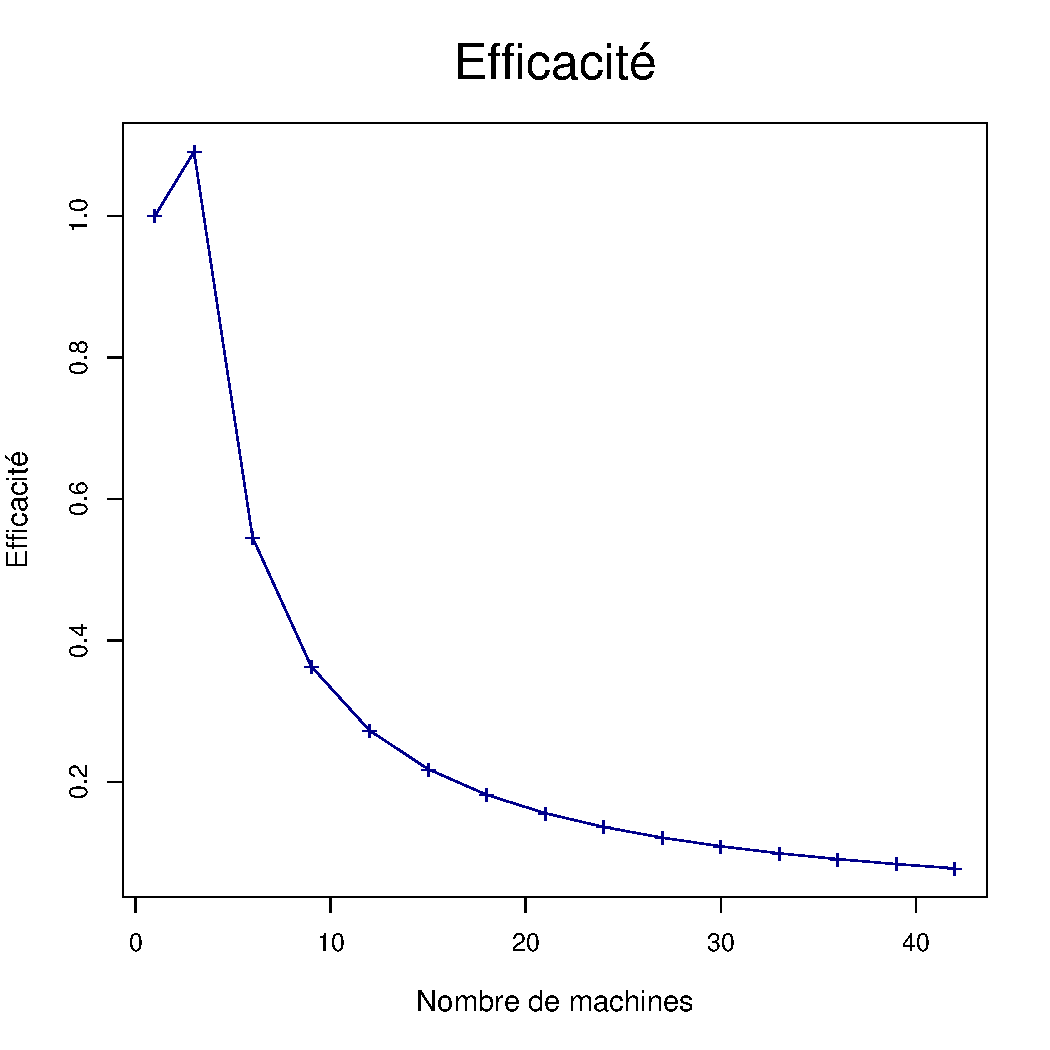
\includegraphics[scale=0.45]{res/sujet_makefiles_premier_Makefile_nth8_eff.pdf}
    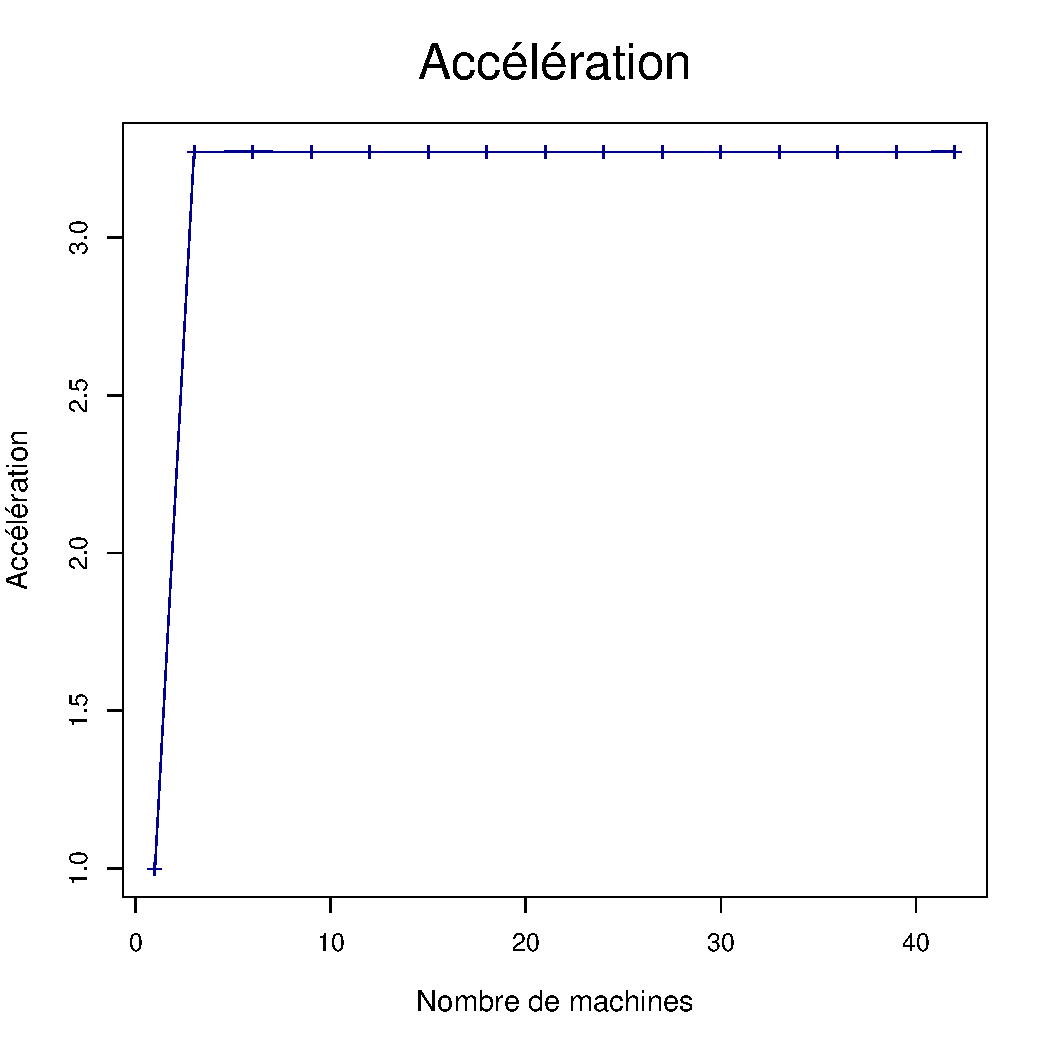
\includegraphics[scale=0.45]{res/sujet_makefiles_premier_Makefile_nth8_acc.pdf}
% \caption{Diagramme des cas d'utilisation}
% \end{figure}
\end{center}

\subsection {Analyse}

Les courbes expérimentales obtenues semblent être plutôt homogènes. Quelques points semblent néanmoins étranges puisqu'ils induisent une augmentation pour un point lorsque l'on attend une diminution. Cela peut s'expliquer par l'incertitude des mesures expérimentales. Cela peut également s'expliquer par l'une des extensions que nous avons réalisées : lorsque l'on envoie une tache à un esclave, on ne renvoie pas les dépendances qu'on lui a déjà précédemment envoyé. En rajoutant des machines on diminue la probabilité de renvoyer à un esclave une tache pour laquelle il a déjà reçu des dépendances ce qui augmente le temps réseau (cette optimisation est moins efficace dans ces cas-là, mais nous obtenons tout de même de meilleurs résultats qu'en ne l'implémentant pas).

On remarque que les courbes expérimentales des temps d'exécution ont la même allure que les courbes théoriques (obtenues en divisant le temps obtenu avec une machine par le nombre de machines). Cependant, de gros écarts apparaissent et croissent avec le nombre de machines. Cela s'explique par le besoin d'envoyer les fichiers sur le réseau et donc par le fait de rajouter du temps d'envoi et de traitement à la fois des fichiers sources, mais aussi des réponses. On remarque que les temps finissent par stagner, souvent aux alentours de 20 machines, car passé ce nombre, il n'y a plus assez de tâches à distribuer et rajouter des esclaves ne fait plus gagner de temps puisque certains esclaves se retrouvent sans tâche à effectuer. En revanche, à partir d'une quarantaine de machines, la tendance est que les temps recommencent à augmenter, car il y a de nombreux esclaves qui demandent des temps de traitement et des temps d'envois réseaux importants (car l'optimisation qui consiste à ne pas renvoyer une dépendance déjà envoyée à un esclave ne marche plus).

Les courbes d'efficacité nous semblent cohérentes, puisqu'elles sont toujours inférieurs à 1 et qu'elles sont décroissantes. Les courbes d'accélérations semblent également globalement cohérentes, puisque rajouter des machines permet d'augmenter l'accélération (représentant le temps gagné en distribuant le makefile plutôt qu'en l'exécutant en séquentiel). Les quelques irrégularités étant dues aux irrégularités des mesures. 


\end{document}


